\documentclass{scndocument}
\pagestyle{plain}
\usepackage{import}
\usepackage{scn} 
\usepackage{multicol}
\usepackage{ragged2e}
\usepackage{amsmath}
\usepackage{setspace}
\usepackage{graphicx}
\graphicspath{{images/}}
\backgroundsetup{contents={}}
\setcounter{page}{87} 
\begin{document}
\begin{SCn}
    \begin{center}
    \huge
 \textbf{Natural Language Text Generation from
Knowledge Bases of ostis-systems}  
\end{center}
\begin{multicols}{3}
\begin{center}
Artem Goylo \par
\textit{Intelligent} \par
\textit{Semantic Systems} \par
Minsk, Belarus \par 
Email: artemgoylo@gmail.com \par
\columnbreak 
Sergei Nikiforov \par
\textit{Belarusian State University of Informatics and Radioelectronics} Minsk, Belarus \par
Email: nikifrov.sergei.al@gmail.com
\columnbreak 
\par
Olga Golovko \par 
\textit{Brest State} \par
\textit{Technical University} \par
Brest, Belarus \par
Email: olechkavgolovko@gmail.com
\end{center}
\end{multicols}
\begin{multicols}{2}
\begin{spacing}{0.65}
\begin{justify} 
\par
\par{\textbf{\textit{Abstract}—The article discusses an approach towards generating coherent natural language texts from fragments of ostis-system knowledge bases. The architecture of the abstract sc-agent of translating a fragment of the knowledge base into a natural language is described. The task of generating a natural language text is subdivided into three sub-tasks: structure filtering, knowledge base fragment decomposition, and generating an equivalent natural language text. Two ways of linearizing a knowledge base fragment are proposed: one based on a predefined order specification and an algorithmic one. Generation of an equivalent natural language text is proposed to be done in two stages. Firstly, an intermediate rough natural language representation is generated using rule-based mappings between sc-text constructions and their corresponding natural language verbalizations. Secondly, the intermediate representation is converted into a coherent natural language text with the help of a large language model. Finally, three possible applications of the proposed approach are described.} \par 
\textbf{\textit{Keywords}—Natural Language Generation, Natural Language Processing, semantic network, Open Semantic Technology for Intelligent Systems (OSTIS), SC-code (Semantic Computer Code), knowledge base, discourse structure}}
\end{justify}
\end{spacing}
\centering {\MakeUppercase{\romannumeral 1}. Introduction}
\setlength{\parindent}{1em}
\begin{justify}
During the last couple of years we have seen a sharp improvement of AI-related technologies. With the rise of Large Language Models (LLMs), automatically generated natural language texts have reached a neverbefore-seen level of adequacy and coherence. However, as it has been well-established, LLMs are prone to hallucinations and factual distortions when generating responses [1]. One of the potential solutions to this problem is using a reliable source of information to provide verified information as context for an LLM (for example, see [2]). Knowledge bases can serve as such a reliable source of information.\par
The OSTIS Technology (Open Semantic Technology for Intelligent Systems) [3] is a technology of complex support of the next-generation intelligent computer systems development life cycle. The technology is particularly focused on using knowledge bases as the core of intelligent computer systems, which are called ostissystems in the context of the technology.\par 
\columnbreak The foundation of the OSTIS Technology is a universal means of semantic representation (coding) of information in the memory of intelligent computer systems, called sc-code. Texts in sc-code (sc-texts and scconstructions) are unified semantic networks that have a basic set-theoretic interpretation. The elements of such semantic networks are called sc-elements (sc-nodes and sc-connectors, which, depending on whether they are directed or not, are called sc-arcs or sc-edges). The universality and unified nature of sc-code allow to use it in order to describe all kinds of knowledge and problemsolving methods, which, in turn, considerably reduces the difficulty of integrating methods and knowledge within a system as well as within a collective of such systems.\par
As sc-texts are, essentially, semantic networks, it follows that they are non
linear in their nature. This fact posits a particular challenge for the natural language generation task, since an sc-text needs to be linearized before being translated into a natural language text.\par 
The goal of this work is to outline a module for generating natural language texts based on both complete and self-contained fragments of a knowledge base, as well as arbitrarily chosen fragments. This module is envisioned as part of the natural language interface of an ostis-system, described in greater detail in our earlier work [4]. To achieve this, we will have to address the following issues:
\end{justify}
\begin{itemize}
\item Filtering irrelevant parts of an sc-text stored in the knowledge base;
\item Linearization of a non-linear text that is a certain graph structure within the knowledge base; 
\item Translation of a linearized sc-text into a natural language.
\end{itemize}
\vspace{0.5cm}
\centerline{\MakeUppercase{\romannumeral 2}. State of the art} 
\vspace{0.3cm}
\setlength{\parindent}{1em}
\begin{justify}
Automatic natural language text generation is a wellresearched problem, with many different approaches having been proposed for solving it.
\par Traditional approaches usually based their natural language generation systems on the rules which were developed using the various theories of discourse structure, 
\end{justify}
\newpage
\setlength{\parindent}{1em}
\begin{justify}
in particular, Rhetorical Structure Theory [5], which
establishes 25 relations that bind sentences within a text
segment. Such approaches usually formalize texts as trees
whose nodes are specific text segments that are partitioned into smaller segments connected via a particular
relation, with leaves of such trees being particular clauses.
An example of an RST-based approach is [6]. Tree-based
representation of texts is in line with such foundational
discourse theories as [7].\\
The issue with the formalisms used by the traditional
approaches is that both discourse macrostructure, as well
as relations between individual sentences, are quite flexible and allow for a certain degree of individual variation.
Besides, the subject domain of rhetorical relations at
the micro-level is not completely formalized, and such
relations can be numerous [6, p. 17], which complicates
the development of natural language generation systems.
On the other hand, some theories emphasize the impossibility of a complete account of relations that hold
between text segments and propose a limited set of basic
relations that are usually structural, rather than semantic
or rhetorical [8].\\
Of the traditional approaches to natural language generation, our approach, which will be described below,
is most similar to [9]. This approach utilizes a formal
model of discourse strategies to generate coherent natural
language texts. Prior to text generation, knowledge is
extracted from a knowledge base, after which its relevancy is established and irrelevant parts are removed.
The approach focuses on generating a coherent text as
a response to a certain question, which is why it needs
to establish relevancy of knowledge found in the knowledge base. The authors define three types of questions:
questions about information available in the knowledge
base, questions about definitions, and questions about
differences between entities in the knowledge base [9,
p. 7]. Text is linearized according to the chosen discourse
strategy, and there is no predefined discourse structure
available in the knowledge base [9, p. 8]. Such an
approach allows to generate variable surface structures
describing the same knowledge representation due to the
focus on discourse strategies [9, p. 9]. Discourse structure
is formalized as specific patterns of usage of rhetorical
predicates (overall 16 such predicates are defined, e.g. attributive, equivalent, specification, explanation, evidence,
analogy, etc.)\\ 
Modern approaches focus on using the latest achievements in the field of AI, in particular, neural networks.
Among them, one popular way of generating natural
language texts is by using some intermediate semantic
representation: for example, formalisms of Discourse
Representation Theory [10], [11]. An approach that is
similar to ours is the variant of translating RDF-triples
into a natural language text, proposed in [12].\\ 
However, a significant number of works within such
approaches focuses on sentence-level generation, rather
than document-level generation. At the same time, approaches that emphasize document-level generation [10],
[11], though acknowledging the task of text linearization
(i. e. ordering of text segments), focus more on solving
particular problems at the sentence-level connected with
the chosen semantic formalism, such as variable naming.\\ 
Still other neural network-based approaches do not use
intermediate semantic representation in natural language
generation, see, for example, [13]. However, pure neural
approaches sometimes have to contend with the issue
that high-level semantic relations, which are important
to capture when generating a coherent natural language
text, present a challenge for neural networks [13, p. 1]
\end{justify}
\vspace{0.3cm}
\centerline{\MakeUppercase{\romannumeral 1}. Suggested approach}
\vspace{0.3cm}
\begin{justify}
We propose to address the issue of generating a
coherent natural language text by adopting a multi-agent
approach to the design of the respective module of natural
language generation based on the OSTIS Technology.\\
The foundation of a knowledge base developed using
the technology is a hierarchical system of semantic models of subject domains and ontologies. An ostis-system
problem solver is represented by a collective of agents
(sc-agents) that interact with each other by specifying the
information processes in the semantic memory that they
execute [14].\\ 
An abstract sc-agent is a certain class of functionally equivalent sc-agents, different instances (i. e. representatives) of which can be implemented in different
ways.[14]\\
Below we will describe our suggested approach by
providing the specifications of agents required for solving
the problem of translating a fragment of the knowledge
base into a natural language text.
The proposed implementation of the agent of translating a fragment of the knowledge base into a natural
language has the following decomposition:
\end{justify} 
\begin{flushleft}
    
\vspace{0.4cm}
\textbf{\textit{Abstract sc-agent of translating a fragment of the knowledge base into a natural language}}
\end{flushleft}
\begin{spacing}{0.65}
\hspace{-3cm} $\Rightarrow$ {\textit{abstrasct sc-agent decomposition*}}:\par
\begin{itemize}
\itemsep0em
\vspace{-0.3cm}
\item [\{ \bullet] \textit{Abstract sc-agent of structure filtering} \leftskip=2em  
\item \textit{Abstract sc-agent of fragment \\ decomposition}
\item \textit{Abstract sc-agent of generating an \\ equivalent natural language text}
\end{itemize}
\vspace{-0.3cm}
\hspace{1cm}$\Rightarrow$ {\textit{abstrasct sc-agent decomposition*}}:
\begin{itemize} \leftskip=7em
\itemsep0em
\vspace{-0.3cm}
\item [\{ \bullet] \textit{Abstract sc-agent of \\ generating a rough version \\ of a natural language text}
\item  \textit{Abstract sc-agent of \\ converting the rough \\ version into a correct \\ natural language text}
\end{itemize}
\end{spacing}
\newpage
\hspace{-2cm}\} \par
\hspace{-6cm} \} \par
\begin{justify}
The agents that are part of this abstract sc-agent will
be discussed below. We will also discuss the agent of
structure filtering that may be used in order to remove
specified parts of a fragment before translating it into
a natural language. The introduction of such an agent
is explained by the fact that the structures that are
to be translated (e. g., the semantic neighborhood of
a certain concept) could be quite large and/or include
irrelevant information, which would lead to a bloated
natural language text that would be more difficult to
comprehend.\par
\end{justify}
\begin{flushleft}
\textit{A. Abstract sc-agent of structure filtering}
\end{flushleft}
\begin{justify}
\setlength{\parindent}{1em}
The input of this agent is the structure to be filtered, and the output of it is a certain subset of the structure.\par The filtering is done by using templates. Two kinds of template sets are proposed: the set of exclusive templates, i.e. the templates that are used to exclude a part of the structure before translation, and the set of inclusive templates, i. e. the ones that specify what part of the structure needs to be kept.\par If a set of inclusive templates is passed to the filtering agent then only the corresponding part of the structure will be outputted. If exclusive templates are used then only the part that does not fit the template will be translated.\par It is also necessary to introduce additional logic — the agent needs to check for connections between the elements of the part to be excluded and the part that is to be kept.\par 
For example, let us consider the situation in figure 1.
\end{justify}
\centering
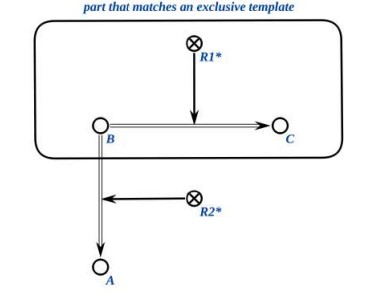
\includegraphics[width=\linewidth]{zzzzzzzzzzzz.jpg}
\caption{\small Figure 1. An example of a structure prior to filtering.}
\begin{justify} 
Here, it is expected that what will be left after filtering
is the fragment of the structure in figure 2: even though
the node B was part of the pattern found using an
exclusive template, it still has a connection with the part
\end{justify}
\centering
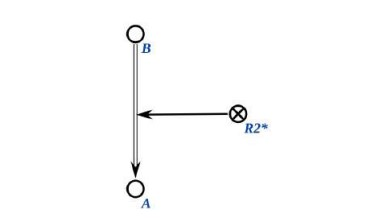
\includegraphics[width=\linewidth]{Снимок экрана 2024-09-16 091549.jpg}
\caption {\small Figure 2. An example of the result of filtering.}
\begin{flushleft}
\textit{B. Abstract sc-agent of fragment decomposition}
\end{flushleft}
\begin{justify}
The goal of this agent is decomposing a fragment of
the knowledge base into an ordered set of substructures.
The order of the substructures indicates the ordering of
the content of each structure during after translation.\par
Classic works on discourse structure note that the
structure of specific discourses depends on their genre
(e. g., a story and a scientific paper will have different
structures) [7]. Thus, different fragments of the knowledge base can have their own respective canonical structures. Hence it is important to discuss, which fragments
of ostis-system knowledge bases are most likely to be
translated into a natural language, and to formalize their
structure.\par
The structure of a text depends on the class of the
structure to be translated and the purpose of its translation, i. e. to what kind of message it can be used as a
response.\par
The input of the agent is a structure to be translated,
while the output is an ordered set of substructures that
is the decomposition of the original structure.
This set of substructures is obtained in two stages:
\end{justify}
\begin{itemize}
\item firstly, a predefined text structure specification is
used;
\item secondly, the ordering of elements within the substructures is derived algorithmically.
\end{itemize}
\begin{justify}
At the first stage, we propose to use a predefined
specification of ordering of substructures stored in the
knowledge base. The substructures are assumed to be
the partition of the original structure (fragment) in the
knowledge base. Such specifications can be defined for
sc-texts of subject domains and other frequently used
fragments of the knowledge base.\par
For example, we propose that a subject domain has
a specification that includes the next elements in the
following order: classes of objects of research (first,
maximal classes and then non-maximal ones), explored
\end{justify}
\end{multicols}
\end{SCn}
\end{document}